\documentclass[tikz,border=3pt]{standalone}
\usetikzlibrary{arrows.meta,positioning,calc}
\hyphenpenalty=10000
\exhyphenpenalty=10000

\begin{document}
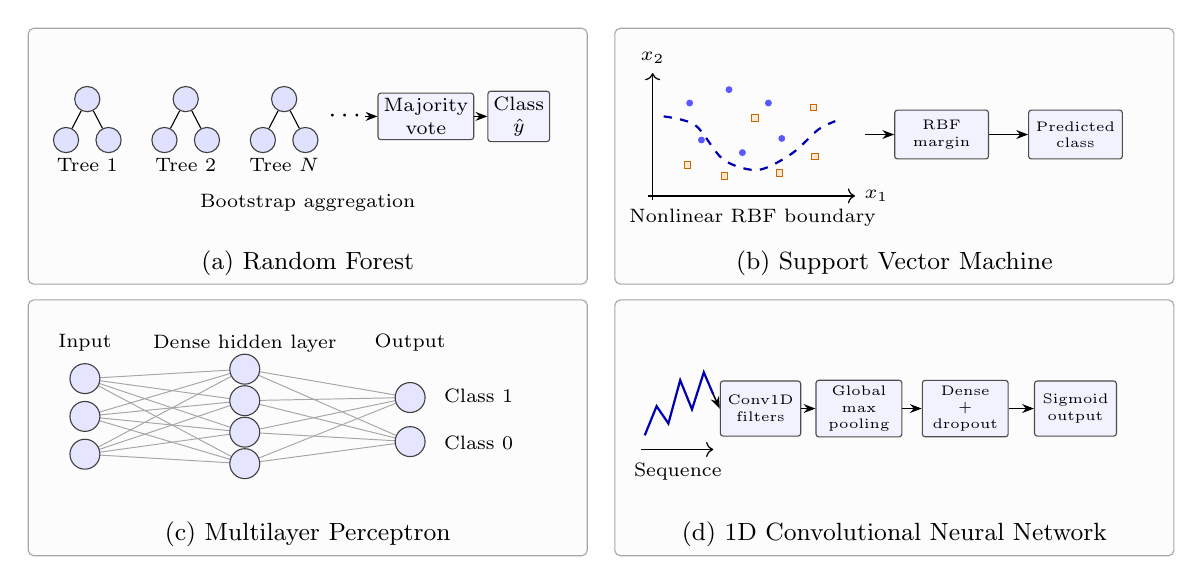
\begin{tikzpicture}[
  panel/.style={draw=black!35,rounded corners=2pt,fill=black!1},
  arrow/.style={-{Stealth[length=1.5mm]},line width=0.55pt},
  split/.style={circle,draw=black!75,fill=blue!12,inner sep=0pt,minimum size=3.2mm},
  neuron/.style={circle,draw=black!75,fill=blue!10,inner sep=0pt,minimum size=3.8mm},
  label/.style={font=\scriptsize,align=center},
  panelcaption/.style={font=\small,align=center},
  flowbox/.style={draw=black!70,rounded corners=1pt,fill=blue!5,align=center,font=\scriptsize,inner sep=2pt}
]

% (a) Random Forest: bootstrap trees aggregate their class votes.
\begin{scope}
  \path[panel] (0,0) rectangle (7.1,-3.25);
  % Tree 1
  \node[split] (rf1r) at (0.75,-0.90) {};
  \node[split] (rf1l) at (0.48,-1.42) {};
  \node[split] (rf1q) at (1.02,-1.42) {};
  \draw (rf1r) -- (rf1l); \draw (rf1r) -- (rf1q);
  \node[label] at (0.75,-1.73) {Tree 1};
  % Tree 2
  \node[split] (rf2r) at (2.00,-0.90) {};
  \node[split] (rf2l) at (1.73,-1.42) {};
  \node[split] (rf2q) at (2.27,-1.42) {};
  \draw (rf2r) -- (rf2l); \draw (rf2r) -- (rf2q);
  \node[label] at (2.00,-1.73) {Tree 2};
  % Tree N
  \node[split] (rf3r) at (3.25,-0.90) {};
  \node[split] (rf3l) at (2.98,-1.42) {};
  \node[split] (rf3q) at (3.52,-1.42) {};
  \draw (rf3r) -- (rf3l); \draw (rf3r) -- (rf3q);
  \node[label] at (3.25,-1.73) {Tree $N$};
  \node at (4.02,-1.12) {$\cdots$};
  \node[flowbox,minimum width=1.05cm,minimum height=0.58cm] (rfvote) at (5.05,-1.12) {Majority\\vote};
  \node[flowbox,minimum width=0.72cm,minimum height=0.58cm] (rfout) at (6.23,-1.12) {Class\\$\hat y$};
  \draw[arrow] (4.28,-1.12) -- (rfvote.west);
  \draw[arrow] (rfvote.east) -- (rfout.west);
  \node[label] at (3.55,-2.22) {Bootstrap aggregation};
  \node[panelcaption] at (3.55,-2.98) {(a) Random Forest};
\end{scope}

% (b) RBF-SVM: nonlinear boundary in the input space, followed by a margin decision.
\begin{scope}[shift={(7.45,0)}]
  \path[panel] (0,0) rectangle (7.1,-3.25);
  \draw[->,line width=0.45pt] (0.42,-2.13) -- (3.05,-2.13) node[right,font=\scriptsize] {$x_1$};
  \draw[->,line width=0.45pt] (0.48,-2.18) -- (0.48,-0.57) node[above,font=\scriptsize] {$x_2$};
  % Two classes in a nonlinear arrangement.
  \foreach \x/\y in {0.95/-0.95,1.45/-0.78,1.95/-0.95,1.10/-1.42,1.62/-1.58,2.12/-1.40}
    \fill[blue!65] (\x,\y) circle (1.25pt);
  \foreach \x/\y in {0.88/-1.78,1.35/-1.92,2.05/-1.88,2.50/-1.67,2.48/-1.05,1.74/-1.18}
    \draw[orange!80!black,fill=orange!18] (\x,\y) rectangle +(2.4pt,2.4pt);
  \draw[blue!70!black,dashed,line width=0.8pt]
    plot[smooth] coordinates {(0.62,-1.12) (1.02,-1.23) (1.38,-1.67) (1.82,-1.80) (2.25,-1.59) (2.58,-1.29) (2.80,-1.18)};
  \node[label] at (1.75,-2.40) {Nonlinear RBF boundary};
  \node[flowbox,font=\tiny,text width=1.05cm,minimum height=0.62cm] (svmmargin) at (4.15,-1.35) {RBF\\margin};
  \node[flowbox,font=\tiny,text width=1.05cm,minimum height=0.62cm] (svmout) at (5.85,-1.35) {Predicted\\class};
  \draw[arrow] (3.18,-1.35) -- (svmmargin.west);
  \draw[arrow] (svmmargin.east) -- (svmout.west);
  \node[panelcaption] at (3.55,-2.98) {(b) Support Vector Machine};
\end{scope}

% (c) MLP: one fully connected hidden layer between input and output.
\begin{scope}[shift={(0,-3.45)}]
  \path[panel] (0,0) rectangle (7.1,-3.25);
  \node[label] at (0.72,-0.55) {Input};
  \node[label] at (2.75,-0.55) {Dense hidden layer};
  \node[label] at (4.85,-0.55) {Output};
  \foreach \yi in {-1.00,-1.48,-1.96}
    \foreach \yh in {-0.88,-1.28,-1.68,-2.08}
      \draw[black!35,line width=0.35pt] (0.72,\yi) -- (2.75,\yh);
  \foreach \yh in {-0.88,-1.28,-1.68,-2.08}
    \foreach \yo in {-1.24,-1.80}
      \draw[black!35,line width=0.35pt] (2.75,\yh) -- (4.85,\yo);
  \foreach \y in {-1.00,-1.48,-1.96}
    \node[neuron] at (0.72,\y) {};
  \foreach \y in {-0.88,-1.28,-1.68,-2.08}
    \node[neuron] at (2.75,\y) {};
  \foreach \y in {-1.24,-1.80}
    \node[neuron] at (4.85,\y) {};
  \node[label] at (5.72,-1.22) {Class 1};
  \node[label] at (5.72,-1.82) {Class 0};
  \node[panelcaption] at (3.55,-2.98) {(c) Multilayer Perceptron};
\end{scope}

% (d) 1D-CNN: one temporal convolution, global pooling, and dense classification.
\begin{scope}[shift={(7.45,-3.45)}]
  \path[panel] (0,0) rectangle (7.1,-3.25);
  % Input sequence
  \draw[->,line width=0.45pt] (0.33,-1.90) -- (1.25,-1.90);
  \draw[blue!70!black,line width=0.8pt] plot coordinates {(0.38,-1.72) (0.53,-1.35) (0.68,-1.57) (0.83,-1.02) (0.98,-1.39) (1.13,-0.92) (1.25,-1.20)};
  \node[label] at (0.80,-2.18) {Sequence};
  \node[flowbox,font=\tiny,text width=0.88cm,minimum height=0.70cm] (cnnconv1) at (1.85,-1.38) {Conv1D\\filters};
  \node[flowbox,font=\tiny,text width=0.95cm,minimum height=0.70cm] (cnnpool) at (3.10,-1.38) {Global max\\pooling};
  \node[flowbox,font=\tiny,text width=0.95cm,minimum height=0.70cm] (cnndense) at (4.45,-1.38) {Dense\\+ dropout};
  \node[flowbox,font=\tiny,text width=0.90cm,minimum height=0.70cm] (cnnclass) at (5.85,-1.38) {Sigmoid\\output};
  \draw[arrow] (1.25,-1.20) -- (cnnconv1.west);
  \draw[arrow] (cnnconv1.east) -- (cnnpool.west);
  \draw[arrow] (cnnpool.east) -- (cnndense.west);
  \draw[arrow] (cnndense.east) -- (cnnclass.west);
  \node[panelcaption] at (3.55,-2.98) {(d) 1D Convolutional Neural Network};
\end{scope}
\end{tikzpicture}
\end{document}
